\documentclass[nooutcomes,noauthor,handout,12pt]{ximera}

\graphicspath{  
{./}
{./whoAreYou/}
{./drawingWithTheTurtle/}
{./bisectionMethod/}
{./circles/}
{./anglesAndRightTriangles/}
{./lawOfSines/}
{./lawOfCosines/}
{./plotter/}
{./staircases/}
{./pitch/}
{./qualityControl/}
{./symmetry/}
{./nGonBlock/}
}


%% page layout
\usepackage[cm,headings]{fullpage}
\raggedright
\setlength\headheight{13.6pt}


%% fonts
\usepackage{euler}

\usepackage{FiraMono}
\renewcommand\familydefault{\ttdefault} 
\usepackage[defaultmathsizes]{mathastext}
\usepackage[htt]{hyphenat}

\usepackage[T1]{fontenc}
\usepackage[scaled=1]{FiraSans}

%\usepackage{wedn}
\usepackage{pbsi} %% Answer font


\usepackage{cancel} %% strike through in pitch/pitch.tex


%% \usepackage{ulem} %% 
%% \renewcommand{\ULthickness}{2pt}% changes underline thickness

\tikzset{>=stealth}

\usepackage{adjustbox}

\setcounter{titlenumber}{-1}

%% journal style
\makeatletter
\newcommand\journalstyle{%
  \def\activitystyle{activity-chapter}
  \def\maketitle{%
    \addtocounter{titlenumber}{1}%
                {\flushleft\small\sffamily\bfseries\@pretitle\par\vspace{-1.5em}}%
                {\flushleft\LARGE\sffamily\bfseries\thetitlenumber\hspace{1em}\@title \par }%
                {\vskip .6em\noindent\textit\theabstract\setcounter{question}{0}\setcounter{sectiontitlenumber}{0}}%
                    \par\vspace{2em}
                    \phantomsection\addcontentsline{toc}{section}{\thetitlenumber\hspace{1em}\textbf{\@title}}%
                     }}
\makeatother



%% thm like environments
\let\question\relax
\let\endquestion\relax

\newtheoremstyle{QuestionStyle}{\topsep}{\topsep}%%% space between body and thm
		{}                      %%% Thm body font
		{}                              %%% Indent amount (empty = no indent)
		{\bfseries}            %%% Thm head font
		{)}                              %%% Punctuation after thm head
		{ }                           %%% Space after thm head
		{\thmnumber{#2}\thmnote{ \bfseries(#3)}}%%% Thm head spec
\theoremstyle{QuestionStyle}
\newtheorem{question}{}



\let\freeResponse\relax
\let\endfreeResponse\relax

%% \newtheoremstyle{ResponseStyle}{\topsep}{\topsep}%%% space between body and thm
%% 		{\wedn\bfseries}                      %%% Thm body font
%% 		{}                              %%% Indent amount (empty = no indent)
%% 		{\wedn\bfseries}            %%% Thm head font
%% 		{}                              %%% Punctuation after thm head
%% 		{3ex}                           %%% Space after thm head
%% 		{\underline{\underline{\thmname{#1}}}}%%% Thm head spec
%% \theoremstyle{ResponseStyle}

\usepackage[tikz]{mdframed}
\mdfdefinestyle{ResponseStyle}{leftmargin=1cm,linecolor=black,roundcorner=5pt,
, font=\bsifamily,}%font=\wedn\bfseries\upshape,}


\ifhandout
\NewEnviron{freeResponse}{}
\else
%\newtheorem{freeResponse}{Response:}
\newenvironment{freeResponse}{\begin{mdframed}[style=ResponseStyle]}{\end{mdframed}}
\fi



%% attempting to automate outcomes.

%% \newwrite\outcomefile
%%   \immediate\openout\outcomefile=\jobname.oc
%% \renewcommand{\outcome}[1]{\edef\theoutcomes{\theoutcomes #1~}%
%% \immediate\write\outcomefile{\unexpanded{\outcome}{#1}}}

%% \newcommand{\outcomelist}{\begin{itemize}\theoutcomes\end{itemize}}

%% \NewEnviron{listOutcomes}{\small\sffamily
%% After answering the following questions, students should be able to:
%% \begin{itemize}
%% \BODY
%% \end{itemize}
%% }
\usepackage[tikz]{mdframed}
\mdfdefinestyle{OutcomeStyle}{leftmargin=2cm,rightmargin=2cm,linecolor=black,roundcorner=5pt,
, font=\small\sffamily,}%font=\wedn\bfseries\upshape,}
\newenvironment{listOutcomes}{\begin{mdframed}[style=OutcomeStyle]After answering the following questions, students should be able to:\begin{itemize}}{\end{itemize}\end{mdframed}}



%% my commands

\newcommand{\snap}{{\bfseries\itshape\textsf{Snap!}}}
\newcommand{\flavor}{\link[\snap]{https://snap.berkeley.edu/}}
\newcommand{\mooculus}{\textsf{\textbf{MOOC}\textnormal{\textsf{ULUS}}}}


\usepackage{tkz-euclide}
\tikzstyle geometryDiagrams=[rounded corners=.5pt,ultra thick,color=black]
\colorlet{penColor}{black} % Color of a curve in a plot



\ifhandout\newcommand{\mynewpage}{\newpage}\else\newcommand{\mynewpage}{}\fi

\title{In the wild}

\author{Bart Snapp}

\begin{document}
\begin{abstract}
  Let's witness the effects of scaling in the wild on actual
  real-world objects.
\end{abstract}
\maketitle


\begin{listOutcomes}
\item Work with real-world numbers.
\item Work with percent increase and percent decrease.
\item Organize and accommodate data.
\item Apply the relation between linear scaling and area scaling.
\item Apply the relation between linear scaling and volume scaling.
\item Translate classroom mathematics into real world mathematics. 
\item Accommodate real-world issues that disrupt theoretical predictions.
\end{listOutcomes}


%% dog house
%% dog crate
%% shoes
%% clothing
%% paint tubes
%% food supplies
%% christmas tree lights
%% wall paper

%% ADD VOLUME TO DOG HOUSE

%% PIZZAS
%% TRASH CANS
%% FURNITURE
%% DOG BEDS
%% Mattresses

\mynewpage



%% ADD VOLUME TO DOG HOUSE


\begin{question}
  I was browsing the INTERNET for a dog house. They come in different
  sizes.
  \begin{center}
    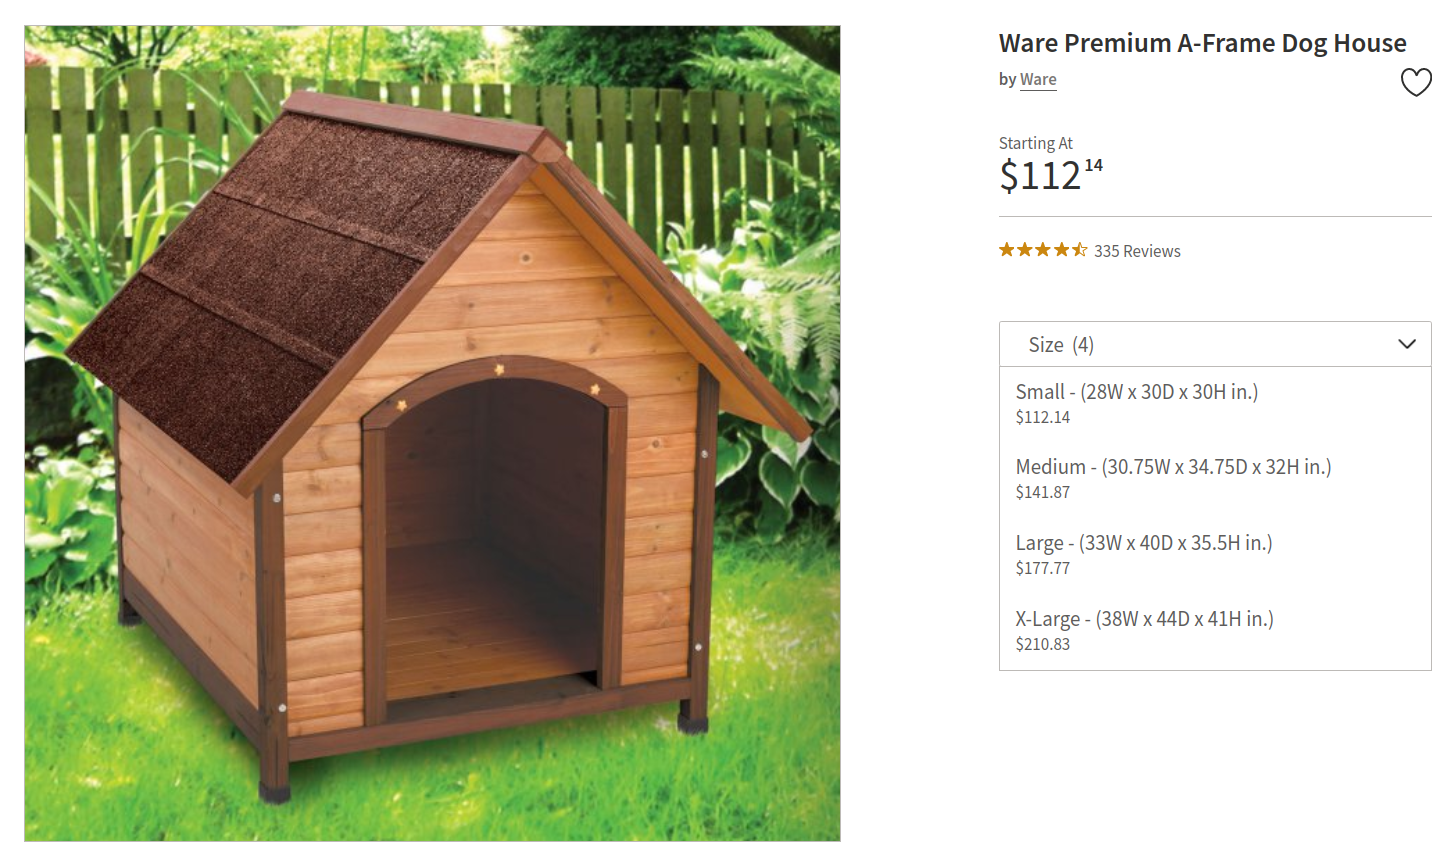
\includegraphics[width=.9\textwidth]{dogHouse.png}
  \end{center}
    \begin{enumerate}
  \item Complete the table below. As a gesture of friendship, I've
    completed some of the columns for you.
    \[
    \renewcommand{\arraystretch}{3}
    \begin{array}{|c||c|c|c|c|c|}
      \hline
      \text{House size} & \text{Width} & \text{Depth} & \text{Height} & \text{Surface area of BOX} & \text{Price} \\ \hline\hline
      \text{Small} & 28    & 30  & 30  & 5160 &    112.14 \\ \hline
      \text{Medium} & 30.75 & 34.75    &  32   &      &    141.87       \\ \hline
      \text{Large} & 33    & 40   & 35.5    &     &     177.77      \\ \hline
      \text{X-Large} & 38    & 44    &  41   &      &    210.83       \\ \hline
    \end{array}
    \]

    \break
    
  \item Find the percent increase of each value in the table above. As
    a gesture of friendship, I've filled in the top and bottom rows.
    \[
    \renewcommand{\arraystretch}{3}
    \begin{array}{|c||c|c|c|}
      \hline
      \text{PERCENT INCREASE} & \text{Small} \to \text{Medium} & \text{Medium}\to\text{Large} & \text{Large}\to \text{X-Large} \\ \hline\hline
      \text{Width} & 10\%  & 7\% & 15\%\\ \hline
      \text{Depth} &  &  & \\ \hline
      \text{Height} &  &  & \\ \hline
      \text{Surface Area of BOX} &  &  & \\ \hline
      \text{Price} & 27\% & 25\% & 19\% \\ \hline
    \end{array}
    \]
  \item Finally, let's compare the percent increases that we found in
    the previous problem by looking at RATIOS. Fill in the table
    below. As a gesture of friendship, I've filled in the first column.
    \begin{gather*}
    \renewcommand{\arraystretch}{3}
    \begin{array}{|c||c|c|c|c|}
      \hline
      \text{RATIO} & \frac{\text{Price Increase}}{\text{Width Increase}}  &  \frac{\text{Price Increase}}{\text{Depth Increase}} &  \frac{\text{Price Increase}}{\text{Height Increase}} &  \frac{\text{Price Increase}}{\text{BOX Increase}}\\ \hline\hline
      \text{Small$\to$Medium} & 1.15  &   &  &  \\ \hline
      \text{Medium$\to$Large} & 1.17 &  & & \\ \hline
      \text{Large$\to$X-Large} & 1.03  &  & & \\ \hline
    \end{array}
    \end{gather*}
    \end{enumerate}
    \begin{freeResponse}
      Here are my tables:
      \begin{enumerate}
      \item 
    \[
    \renewcommand{\arraystretch}{3}
    \begin{array}{|c||c|c|c|c|c|}
      \hline
      \text{House size} & \text{Width} & \text{Depth} & \text{Height} & \text{Surface area of BOX} & \text{Price} \\ \hline\hline
      \text{Small} & 28    & 30  & 30  & 5160 &    112.14 \\ \hline
      \text{Medium} & 30.75 &  34.75   &  32   & 6329     & 141.87          \\ \hline
      \text{Large} & 33    & 40    & 35.5    & 7823     & 177.77          \\ \hline
      \text{X-Large} & 38    & 44    & 41    & 10068     & 210.83          \\ \hline
    \end{array}
    \]
  \item
    \[
    \renewcommand{\arraystretch}{3}
    \begin{array}{|c||c|c|c|}
      \hline
      \text{PERCENT INCREASE} & \text{Small} \to \text{Medium} & \text{Medium}\to\text{Large} & \text{Large}\to \text{X-Large} \\ \hline\hline
      \text{Width} & 10\%  & 7\% & 15\%\\ \hline
      \text{Depth} & 16\% & 15\%  & 10\% \\ \hline
      \text{Height} & 7\%  & 11\%  & 15\%\\ \hline
      \text{Surface Area of BOX} & 23\%  & 24\%  & 29\% \\ \hline
      \text{Price} & 27\% & 25\% & 19\% \\ \hline
    \end{array}
    \]
  \item 
    \[
    \renewcommand{\arraystretch}{3}
    \begin{array}{|c||c|c|c|c|}
      \hline
      \text{RATIO} & \frac{\text{Price Increase}}{\text{Width Increase}}  &  \frac{\text{Price Increase}}{\text{Depth Increase}} &  \frac{\text{Price Increase}}{\text{Height Increase}} &  \frac{\text{Price Increase}}{\text{BOX Increase}}\\ \hline\hline
      \text{Small$\to$Medium} & 1.15  & 1.09   &1.19  & 1.03  \\ \hline
      \text{Medium$\to$Large} & 1.17 &  1.09 & 1.13 & 1.01 \\ \hline
      \text{Large$\to$X-Large} & 1.03  & 1.08 & 1.03 & 0.92\\ \hline
    \end{array}
    \]
    \end{enumerate}
    \end{freeResponse}
\end{question}

\mynewpage



%% \begin{question}
%%   Consider this series of televisions:
%%   \begin{itemize}
%%   \item \url{https://electronics.sony.com/tv-video/televisions/all-tvs/p/xr55x90k}
%%   \end{itemize}
%%   \begin{enumerate}
%%   \item Complete the table below. As a gesture of friendship, I've
%%     completed the first row and column.
%%     \[
%%     \renewcommand{\arraystretch}{3}
%%     \begin{array}{|c|c|c|c|c|}
%%       \hline
%%       \text{Diagonal (cm)} & \text{Area (cm${}^2$)} & \text{Volume (cm${}^3$)} & \text{Mass (kg)} & \text{Price (MSRP in \$)} \\ \hline\hline
%%       139 & 8767 & 63069 & 17.4 & 1299.99 \\ \hline
%%       164 &        &         &      &        \\ \hline
%%       189 &        &         &      &        \\ \hline
%%       215 &        &         &      &        \\ \hline
%%     \end{array}
%%     \]
%%   \item Find the percent increase of each value in the table above.
%%     As a gesture of friendship, I've filled in the top and bottom
%%     rows.
%%         \[
%%     \renewcommand{\arraystretch}{3}
%%     \begin{array}{|c||c|c|c|}
%%       \hline
%%       \text{PERCENT INCREASE} & 139 \to 164 & 164\to 189 & 189\to 215 \\ \hline\hline
%%       \text{Diagonal} & 18\%  & 15\% & 14\%\\ \hline
%%       \text{Area} &  &  & \\ \hline
%%       \text{Volume} &  &  & \\ \hline
%%       \text{Mass} &  &  & \\ \hline
%%       \text{Price} & 15\% & 33\% & 50\% \\ \hline
%%     \end{array}
%%     \]
%%   \item  Finally, let's compare the percent increases that we found in
%%     the previous problem by looking at RATIOS. Fill in the table
%%     below. As a gesture of friendship, I've filled in the top row.
%%     \[
%%     \renewcommand{\arraystretch}{3}
%%     \begin{array}{|c||c|c|c|c|}
%%       \hline
%%       \text{RATIO} & \frac{\text{Price Increase}}{\text{Diagonal Increase}}  &  \frac{\text{Price Increase}}{\text{Area Increase}} &  \frac{\text{Price Increase}}{\text{Volume Increase}} &  \frac{\text{Price Increase}}{\text{Mass Increase}}\\ \hline\hline
%%       139 \to 164 &  0.98  & 0.84 & 0.84 & 0.87 \\ \hline
%%       164\to 189  &  &  &  &  \\ \hline
%%        189\to 215 &  &  &  &  \\ \hline
%%     \end{array}
%%     \]
%%   \end{enumerate}
%%   \begin{freeResponse}
%%     Here are my tables:
%%     \begin{enumerate}
%%     \item 
%%       \[
%%       \renewcommand{\arraystretch}{3}
%%       \begin{array}{|c|c|c|c|c|}
%%         \hline
%%         \text{Diagonal (cm)} & \text{Area (cm${}^2$)} & \text{Volume (cm${}^3$)} & \text{Mass (kg)} & \text{Price (MSRP in \$)} \\ \hline\hline
%%         139 & 8767 & 63069  & 17.4  & 1299.99  \\ \hline
%%         164 & 12110   & 87190   & 22.9  & 1499.99 \\ \hline
%%         189 & 16114   & 117629  & 34.4  & 1999.99 \\ \hline
%%         215 & 20721   & 141263 & 45.8 & 2999.99 \\ \hline
%%       \end{array}
%%       \]
%%     \item 
%%       \[
%%       \renewcommand{\arraystretch}{3}
%%       \begin{array}{|c||c|c|c|}
%%         \hline
%%         \text{PERCENT INCREASE} & 139 \to 164 & 164\to 189 & 189\to 215 \\ \hline\hline
%%         \text{Diagonal} & 18\%  & 15\% & 14\%\\ \hline
%%         \text{Area} &  38\% & 33\%  & 29\% \\ \hline
%%         \text{Volume} & 38\%  & 35\% & 29\% \\ \hline
%%         \text{Mass} & 31\%  & 50\% & 33\%\\ \hline
%%         \text{Price} & 15\% & 33\% & 50\% \\ \hline
%%       \end{array}
%%       \]
%%     \item 
%%       \[
%%       \renewcommand{\arraystretch}{3}
%%       \begin{array}{|c||c|c|c|c|}
%%         \hline
%%         \text{RATIO} & \frac{\text{Price Increase}}{\text{Diagonal Increase}}  &  \frac{\text{Price Increase}}{\text{Area Increase}} &  \frac{\text{Price Increase}}{\text{Volume Increase}} &  \frac{\text{Price Increase}}{\text{Mass Increase}}\\ \hline\hline
%%         139 \to 164 &  0.98  & 0.84 & 0.83 & 0.88 \\ \hline
%%       164\to 189  & 1.16 & 1    & 0.99 & 0.89 \\ \hline
%%       189\to 215 & 1.32  & 1.17 & 1.17 & 1.13 \\ \hline
%%     \end{array}
%%       \]
%%       \end{enumerate}
%%   \end{freeResponse}
%% \end{question}




\begin{question}
  Let's REFLECT on your computations above. In particular, let's
  examine table (c).% from both problems above.
  %\begin{enumerate}
  %\item
  \begin{enumerate}
    \item Which increase: WIDTH, DEPTH, HEIGHT, SURFACE AREA OF BOX;
      is most similar to the increase of the PRICE?
    \item EXPLAIN HOW you identified which increase aligns with the
      increase of the price.
    \item DISCUSS WHY this is the case.
  \end{enumerate}
   % \item Considering the TVs, which increase: DIAGONAL, AREA, VOLUME,
    %  MASS; is most similar to the increase of the PRICE?  EXPLAIN HOW
      %you identified which increase aligns with the increase of the
     % price and DISCUSS WHY this is the case.
  %\end{enumerate}
\end{question}
\mynewpage


\begin{question}
  A lot of common items come in different sizes and the price
  difference is negligible. This is due to the fact that the raw
  materials of objects often don't dictate the price.

  \textbf{Find a real pizza menu. Does the price of pizza scale like the
  diameter, area, or volume?  Explain why this is the case.}
 
\end{question}






\end{document}
